
%(BEGIN_QUESTION)
% Copyright 2014, Tony R. Kuphaldt, released under the Creative Commons Attribution License (v 1.0)
% This means you may do almost anything with this work of mine, so long as you give me proper credit

Calculate the voltage across the resistor in this circuit, as well as its power dissipation:

$$\includegraphics[width=15.5cm]{i00827x01.eps}$$

$V_R$ = \underbar{\hskip 50pt}

\vskip 10pt

$P_R$ = \underbar{\hskip 50pt}

\vskip 10pt

\underbar{file i00827}
%(END_QUESTION)





%(BEGIN_ANSWER)

Here is a helpful hint: draw a phasor diagram of the system voltage first, showing the $-90^{o}$ phasor $V_{AB}$ and the proper phase rotation (ABC, counter-clockwise):

$$\includegraphics[width=15.5cm]{i00827x02.eps}$$

The phasor diagram is shown as a Delta because the only voltage values we've been given are line (i.e. from one phase conductor to the other).  If the given voltage was a phase quantity, it would make most sense to begin by drawing a Wye-shaped phasor diagram showing each voltage as a phasor originating from a center point (ground).

\vskip 10pt

\noindent
{\bf Final answers:}

\vskip 10pt

$V_R = 242.56 \hbox{ V} \angle 148.9^o$

\vskip 10pt

$P_R = 196.1 \hbox{ W}$

%(END_ANSWER)





%(BEGIN_NOTES)

From our initial phasor diagram we may tell that phase B's voltage with reference to ground ($V_B$) is 277.1 volts at an angle of +120 degrees:

$$\includegraphics[width=15.5cm]{i00827x03.eps}$$

This is the voltage powering our series RC network.

\vskip 10pt

Calculating the impedance of the capacitor:

$$X_C = {1 \over 2 \pi f C} = 165.79 \> \Omega$$

$$Z_C = 0 - j165.79 \> \Omega$$

\vskip 10pt

Calculating the impedance of the series RC network:

$$Z_T = Z_C + Z_R$$

$$Z_T = (0 - j165.79 \> \Omega) + (300 + j0 \> \Omega) = 300 - j165.79 \> \Omega = 342.8 \> \Omega \angle -28.93^o$$

\vskip 10pt

Calculating current through the series RC network:

$$I = {V \over Z} = {277.1 \hbox{ V} \angle 120^o \over 342.8 \> \Omega \angle -28.93^o}$$

$$I = 0.8085 \hbox{ A} \angle 148.9^o$$

\vskip 10pt

The resistor's voltage drop is simply this current multiplied by the resistor's impedance:

$$V_R = IZ_R = (0.8085 \hbox{ A} \angle 148.9^o)(300 \> \Omega \angle 0^o)$$

$$V_R = 242.56 \hbox{ V} \angle 148.9^o$$

\vskip 10pt

Power is a scalar calculation, so we take the voltage magnitude squared divided by the resistor's resistance:

$$P_R = {V^2 \over R} = {(242.56 \hbox{ V})^2 \over 300 \> \Omega} = 196.1 \hbox{ W}$$

%INDEX% Electronics review: 3-phase voltage/current/power calculation
%INDEX% Electronics review: AC reactance and impedance
%INDEX% Electronics review, phasor expressions of circuit quantities
%INDEX% Electronics review: series and parallel AC circuits

%(END_NOTES)


